\chapter{Entwicklung eines Frameworks und Durchführung von Experimenten}
Zur Zielsetzung Konfiguartionskonzept, Dinge die fehlen, Ableitung einer Vorgehensweise 

Denn in großen Gebieten, wie z.B. Einkaufshäuser, Lagerhallen und Flughäfen braucht man Hunderte von iBeacons, um die gesamte Fläche zu 100 Prozent abzudecken. Im Idealfall kann ich später in Matlab noch Gebiete einpflegen, an der die Karte nach Regionen aufgeteilt wird, in denen die Genauigkeit der Lokalisierung eingestellt werden kann. Damit ließe sich Robotergestützt ein Gebiet abfahren, in denen Vorschläge für die Positionierung von iBeacons anhand eines Optimierungsalgorithmusses generiert werden. Hierbei ließe sich wunderschön eine Pareto-Front bilden, die aus Anzahl von iBeacons und Genauigkeit pro Region Positionierungsvorschläge entwirft. Je nach Kundenwunsch. ROTER FADEN ZU MEINER ARBEIT!

Hier kann angesprochen werden das wir ein adaptives Verfahren entwickeln wollen, denn viele bisherige Systeme bieten lediglich ein Landmarkenssystem oder ein Positionierungssystem. Mit den Beacons soll beides möglich sei und je nach Kundenwunsch anpassbar werden.

\section{Verwendete Hardware}
\subsection{Motorola Moto G}
Dieses Smartphone dient als Empfangsstation des Beacon-Signale. 
\begin{figure}[H]
\centering
%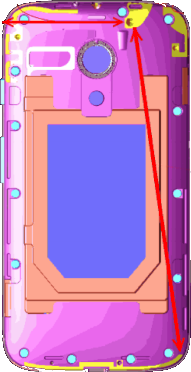
\includegraphics[scale=0.8]{Bilder/MotorolaAntenne}
%\caption{Anordnung der Atennen eines Motorola Moto G  \cite{Moto}}
%\label{fig:Moto}
%\begin{picture}(0,0)
%\put(80,240.5){Bluetooth- und WLAN-Atenne}
%\put(30,245.5){\color{red}\linethickness{0.6mm}\vector(1,0){45}}
%\end{picture}
\begin{tikzpicture}
\node [anchor=south west,inner sep=0] at (0,0) {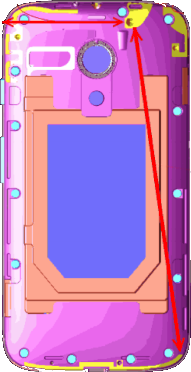
\includegraphics[scale=0.8]{Bilder/MotorolaAntenne}};
\draw [red,->,line width=0.65mm] (3,7.415) -- (4.5,7.415);
\node [anchor=south west,inner sep=0, text width = 4cm] at (5,7) {Bluetooth- und WLAN-Antennen};
\end{tikzpicture}
\caption{Anordnung der Atennen an der Rückseite eines Motorola Moto G  \cite{Moto}}
\label{fig:Moto}
\end{figure}

!Atennencharackteristiken! Idee für die Erklärung der seltsamen Empfangsqualität bei den verschiednen Ausrichtungen: durch die Verteilung der Antennen ergibt sich auch eine Verteilung der Empfangscharackeristiken. Die dabei aufgenommenen Messwerte sehen bei den unterschiedlichen Ausrichtungen deshalb immer gleich aus, auch wenn die Signale aus einer anderen Richtung kommen, weil die Charackteristik speziell auf auf die normale Position optimiert wurde. Durch die Komplexität der Charackteristiken lässt sich dies nun schlecht visuell darstellen. Wenn man das Verhalten aber kennt (vorsicht, jedes Smartphone hat eine unterschiedliche Charakteristik), kann man Gegenmaßnahmen treffen. -> Heuristik 
\subsection{Youbot}
\begin{figure}[H] 
\centering
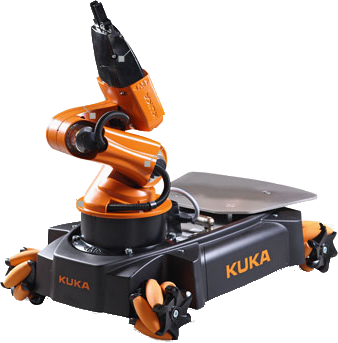
\includegraphics[scale=0.5]{Bilder/Youbot}
\caption{Youbot von Kuka \cite{You}}
\end{figure}
\subsection{Scitos G5}
Bild vom Flur

\section{Verwendete Software}
\subsection{ROS}
\subsection{Android-Studio}
\subsection{Estimote SDK for Android}
\subsection{App-Entwicklung}

\section{Versuchsplanung}
Erklärung der Funktionsweise des Frameworks

\section{Experimente}
\subsection{Energieverbrauch eines Beacon}
Hier wird erklärt, dass sich durch die Einstellmöglichkeiten der Beacons auch deren Energiebedarfs der einzelnen Komponenten ändert (Mikrocontroller, BLE-Modul). Denn bei einer höheren Sendeleistung Verbraucht das BLE-Modul mehr Energie und bei einer Erhöhung der Sendefrequenz verbrauchen BLE-Modul und der Mikrocontroller (muss häufiger "`aufwachen"') mehr. 
Graphik mit Leistungsverbrauch der beacons in Abghängigkeit mit ihren Einstellungen. Die Farbe soll dabei der Leistungsverbrauch und die Achsen die Intervallzeit und die Sendeleistung darstellen. Hier kann man sich auch überlegen die theoretische Akkulaufzeit mit anzugeben. Die Knopfbatterien sind vom Typ CR2450 mit einem Energiegehalt von ca. 1,8 Wh \cite{CR2450}. Der Mikrocontroller kann hier nicht mit eingerehnet werden, da lediglich ein Verbrauch in Abhängigkeit mit der Prozessorgeschwindigkeit \cite{ARM} gegeben ist und für die Beacons keine Informationen vorliegen, in welcher Taktfrequenz diese betrieben werden. Natürlich hat der Prozessor auch eine höhere Taktfrequenz, wenn die Sendeintervalle der Beacons häufiger stattfinden und somit ist beides aneinander gekoppelt. Deswegen Messung des Stromverbrauchs am Beacon bei minimaler Sendeleistung mit den unterschiedlichen Intervallen (niedrigster Stufe, mittlerer und höhster) und dann einfach linear approximieren.
Bei einer angenommenen Datenrate von 250Kbit/s \cite{nRF5} und bei einer Größe eines Datenpaketes von 30 Bytes \cite{iBPa} (siehe \ref{fig:iBPa}), dauert eine Sendesequenz ca. 0,96 ms. Da für den Sendevorgang noch zusätzlich der Cortex M0 Prozessor aufgeweckt werden muss und dieser das Paket vorbereitet und bis zum Ende der Sendung abwartet, muss hierfür zusätzlich der Energieverbrauch berechnet werden. Da eine direkte Leistungsmessung an den Beacons durch die gering fließenden Ströme nicht möglich ist, werden aus dem Datenblatt des Prozessors diese rechnerisch ermittelt. Die wache Phase des Prozessors für alle Operationen vor und nach einer Sendung werden dabei mit 1,4 ms Sekunden angenommen, was jedoch sehr großzügig bemessen ist und in der Realität weit darunter liegen wird. Der Energiebedarf ist im Datenblatt mit 5,1 $\mu$W/MHz angegeben und auf dem Beacon wurde ein zu 16 MHz oszillierender Quarz verbaut, sodass dieser als Taktgeber verwendet wird. So ergibt sich eine verbrauchte Leistung für eine Sendung zu 0,4 $\mu$Ws.
\begin{figure}[H]
\centering
\begin{tikzpicture}
    \node [block, fill=magenta!20, text width=2cm, minimum height=1.5cm] (Header) {\small Header \\(2 Bytes)};
    \node [block, fill=magenta!20, right=0cm of Header, text width=3cm, minimum height=1.5cm] (MAC) {\small MAC Addresse \\(6 Bytes)};
    \node [block, fill=magenta!20, right=0cm of MAC, text width=2cm, minimum height=1.5cm] (Data) {\small Data \\(30 Bytes)};
    \node [block, fill=blue!20, below=1cm of Data, text width=2cm, minimum height=1.5cm] (Major) {\small Major\\ (2 Bytes)};
    \node [block, fill=blue!20, left=0cm of Major, text width=3cm, minimum height=1.5cm] (UUID) {\small Proximity UUID \\(16 Bytes)};
    \node [block, fill=blue!20, left=0cm of UUID, text width=3cm, minimum height=1.5cm] (Prefix) {\small iBeacon Prefix \\(9 Bytes)};
    \node [block, fill=blue!20, right=0cm of Major, text width=2cm, minimum height=1.5cm] (Minor) {\small Minor\\ (2 Bytes)};
    \node [block, fill=blue!20, right=0cm of Minor, text width=2cm, minimum height=1.5cm] (TX) {\small TX Power\\ (1 Bytes)};
    \draw[very thick,->] (Data) -- (Major);
\end{tikzpicture}
\caption{Anteile eines Datenpaket in der Beacon-Kommunikation auf der MAC-Ebene}
\label{fig:iBPa}
\end{figure}
\subsection{Distanzmessung mithilfe von Beacons}
Zuerst werden zwei bis drei Distanzen und dazu die berechnete Distanz aus der App gegenübergestellt. Das wird schlecht sein und aus dem weitren Grund, dass es eine "`Black Box"' ist (d.h. man kann nicht einsehen, wie die Distanz aus dem RSSI-Wert berechnet wird), wird hier geplant ein eigenes Modell aufzustellen. Da wurde entschieden für verschiedene Distanzen nur die RSSI-Werte aufzunehmen, um später ein eigenes Modell zu implementieren.
\subsection{Einfluss der Sendefrequenz} 
Wird das Rauschen vermindern.
\subsection{Einfluss der Signalstärke} 
Dies soll auch in Abhängigkeit zur Signalsstärke passieren, um dessen Ausbreitung zu erforschen.
\subsection{Auswirkung der Smartphone-Ausrichtung auf die Messungen}
Hier kommen mal alle Messungen rein. Auch die mit den Beacons an allen drei Himmelsrichtungen.
\subsection{Einfluss anderer Funkquellen auf die RSSI-Messung} 
Für die Erklärung aus dem zweiten Kapitel (2,4 Ghz) benötige ich auch die Störung und Interferenzen gleicher Signale. Ich muss ja schließlich erklären, warum ich nicht viele viele iBeacons nebeneinander klatschen kann, um eine möglichst genaue Standortbestimmung zu erhalten (denn die Signale stören sich untereinander). 
ir ist z.B. aufgefallen, dass die Beacons sich gegenseitig in der Sendestärke beeinflussen. Deswegen musste ich Einzelmessungen vornehmen und hier ließe sich auch begründen nicht zu viele Beacons in der realen Anwendung zu plazieren, um durch Elektrosmog nicht zu viele Einflussfaktoren in die Lokalisierung miteinfließen zu lassen. Viel hilft hier nicht immer viel, weniger ist manchmal besser, etc.